% Created 2023-01-12 Πεμ 22:22
% Intended LaTeX compiler: pdflatex
\documentclass[11pt]{article}
\usepackage[utf8]{inputenc}
\usepackage[T1]{fontenc}
\usepackage{graphicx}
\usepackage{longtable}
\usepackage{wrapfig}
\usepackage{rotating}
\usepackage[normalem]{ulem}
\usepackage{amsmath}
\usepackage{amssymb}
\usepackage{capt-of}
\usepackage{hyperref}
\usepackage{booktabs}
\usepackage{import}
\usepackage[LGR, T1]{fontenc}
\usepackage[greek, english]{babel}
\usepackage{alphabeta}
\usepackage{esint}
\usepackage{mathtools}
\usepackage{esdiff}
\usepackage{makeidx}
\usepackage{glossaries}
\usepackage{newfloat}
\usepackage{minted}
\usepackage{chemfig}
\usepackage{svg}
\usepackage[a4paper, margin=3cm]{geometry}
\author{Βιδιάνος Γιαννίτσης}
\date{\today}
\title{Ανάλυση του block 100 - Steam Explosion}
\hypersetup{
 pdfauthor={Βιδιάνος Γιαννίτσης},
 pdftitle={Ανάλυση του block 100 - Steam Explosion},
 pdfkeywords={},
 pdfsubject={},
 pdfcreator={Emacs 28.2 (Org mode 9.5.5)}, 
 pdflang={English}}
\makeatletter
\newcommand{\citeprocitem}[2]{\hyper@linkstart{cite}{citeproc_bib_item_#1}#2\hyper@linkend}
\makeatother

\usepackage[notquote]{hanging}
\begin{document}

\maketitle
\tableofcontents

\renewcommand{\abstractname}{Περίληψη}
\renewcommand{\tablename}{Πίνακας}
\renewcommand{\figurename}{Σχήμα}
\renewcommand\listingscaption{Κώδικας}

\section{Διάγραμμα ροής και επεξήγηση}
\label{sec:orgab1a710}
\begin{figure}[htbp]
\centering
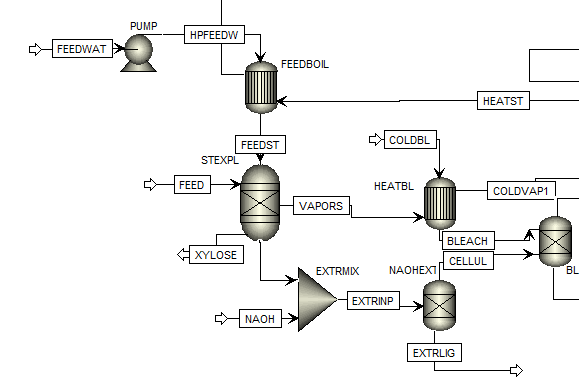
\includegraphics[width=.9\linewidth]{/home/vidianos/Documents/7o_εξάμηνο/Σχεδιασμός_Ι/Project/git_repo/Final_exam_files/Block_100_-_Steam_Explosion/2023-01-10_18-30-22_screenshot.png}
\caption{Διάγραμμα ροής του block 100}
\end{figure}

Στο block 100 γίνεται η αρχική τροφοδοσία της διεργασίας (πυρηνόξυλο) και η κλασματοποίηση του στα 3 βασικά του στοιχεία, την κυτταρίνη, την ημικυτταρίνη και την λιγνίνη. Στο διάγραμμα ροής φαίνεται η παραγωγή ατμού υψηλής πίεσης ο οποίος οδηγείται μαζί με το πυρηνόξυλο στην διεργασία της έκρηξης ατμού. Ο ατμός αυτός παράγεται χρησιμοποιώντας τον ατμό υψηλής πίεσης που παράγεται στον λέβητα της εγκατάστασης (block 300). Από την έκρηξη ατμού (steam explosion) βγαίνουν 3 ρεύματα. Το ημικυτταρινικό κλάσμα με κύριο συστατικό την ξυλόζη (XYLOSE στο διάγραμμα), το στερεό κλάσμα της κυτταρίνης και της λιγνίνης και οι ατμοί οι οποίοι οφείλονται κυρίως σε ότι διασπάστηκε θερμικά και απελευθερώθηκε ως υδρατμοί, διοξείδιο του άνθρακα και άζωτο.

Έπειτα, τα στερεά αναμιγνύονται με υδατικό διάλυμα NaOH και οδηγούνται σε μία διάταξη εκχύλισης στερεού-υγρού στην οποία απομακρύνεται μεγάλο ποσοστό της λιγνίνης. Επειδή δεν απομακρύνεται όλη όμως και η ύπαρξη της στην τροφοδοσία του block 200 μειώνει την ταχύτητα καθώς και την απόδοση της διεργασίας, ακολουθεί και ένα bleacher με NaClO το οποίο απομακρύνει όλη την ποσότητα λιγνίνης.

Μία παράβλεψη που έχει γίνει είναι ότι αν δεν ψυχθεί το ρεύμα των στερεών μετά την έκρηξη ατμού, κατά την ανάμιξη του με το υδατικό διάλυμα, μπορεί αυτό να εξατμιστεί, με αποτέλεσμα να μην έχουμε ακριβώς ανάμιξη υγρού-στερεού, αλλά στερεού-αερίου. Για αυτό, πρέπει να ψυχθεί αυτό το ρεύμα. Επίσης, το ρεύμα αυτό καταλήγει μετά από μερικές διεργασίες στο block 200 όπου ψύχεται για να μπεί στον αντιδραστήρα της ενζυμικής υδρόλυσης. Άρα, θα ήταν καλύτερη ίδεα να υπάρχει εδώ ένας ψυκτήρας, το οποίο όμως δεν έχει διορθωθεί λόγω χρόνου.

\section{Σχεδιαστικές Επιλογές}
\label{sec:orgc895b87}
Η βασικότερη σχεδιαστική επιλογή του block 100 αφορά την έκρηξη ατμού και συγκεκριμένα τον ατμό που χρησιμοποιείται σε αυτήν. Στην βιβλιογραφία, βρέθηκε μία εκτενή λίστα πειραμάτων έκρηξης ατμού σε πυρηνόξυλο για διαφορετικές συνθήκες, αναφέροντας σε κάθε περίπτωση τα yields της διεργασίας \textsuperscript{\citeprocitem{1}{1}} . Συγκρίνοντας τις επιλογές με σκοπό την μεγιστοποίηση της γλυκόζης και ξυλόζης που μπορούν να παραχθούν σε σχέση με την αρχική σύσταση του πυρηνόξυλου σε κυτταρίνη και ημικυτταρίνη, αποφασίστηκε πως η χρήση υπέρθερμου ατμού στα 26 bar και 232 \(^oC\) είναι η ιδανική. Άλλη σημαντική σχεδιαστική επιλογή είναι οι διαχωρισμοί που θα χρησιμοποιηθούν. Η εκχύλιση με υδατικό διάλυμα NaOH είναι μία άρκετά κλασσική διεργασία για τον διαχωρισμό της λιγνίνης από την κυτταρίνης, αλλά δεν μπορεί να απομακρύνει όλη την λιγνίνη με αποτέλεσμα να περισσεύει αρκετή στο ρεύμα της κυτταρίνης \textsuperscript{\citeprocitem{1}{1},\citeprocitem{2}{2}} .

Η σχεδιαστική επιλογή έγκειται στο αν θέλουμε να χρησιμοποιήσουμε αυτό το ρεύμα όπου ξέρουμε ότι η λιγνινή θα δράσει ανασχετικά για τις κυτταρινάσες κατά την υδρόλυση της κυτταρίνης αλλά δεν θα έχει τόσο σημαντική επίδραση εφόσον διαχωρίστηκε σε καλό βαθμό ή αν θέλουμε να κάνουμε ένα παραπάνω βήμα ώστε να απομακρύνουμε όλη την λιγνίνη και να πετύχουμε την μέγιστη δυνατή απόδοση. Το επιπλέον βήμα είναι ένα στάδιο bleaching με ελαφρώς όξινο (με οξικό οξύ) υδατικό διάλυμα NaClO\textsubscript{2}. Με βάση την σχετική βιβλιογραφία, η διεργασία αυτή διώχνει όλη την υπολοιπόμενη λιγνίνη με αποτέλεσμα να έχουμε ένα καθαρό ρεύμα κυτταρίνης \textsuperscript{\citeprocitem{2}{2},\citeprocitem{3}{3}} .

Επίσης βέβαια, έχει σημασία και τι ποσότητα χρειάζεται από τα αντιδραστήρια αυτά για την διεργασία. Γενικά και τα δύο χρειάζονται σχετικά μικρή ποσότητα. Για την εκχύλιση επιλέχθηκε μία παροχή 25 L/min ώστε η μολαρική παροχή του να είναι ίδιας τάξης μεγέθους με αυτήν των στερεών. Το NaOH προτείνεται να είναι της τάξης του \(2 \% \frac{w}{w}\) \textsuperscript{\citeprocitem{1}{1}}. Με παρόμοιο κριτήριο, στο bleaching θα χρησιμοποιηθεί ένα κυβικό μέτρο νερό. Για να πετύχουμε την σύσταση που αναφέρεται στην βιβλιογραφία, σε αυτό θα προστεθούν 20.5 kg NaClO\textsubscript{2} και 6.96 g Οξικό οξύ και το μίγμα θα θερμανθεί στους 70 \(^oC\) (χρησιμοποιόντας την περίσσεια θερμική ενέργεια των ρευμάτων του steam explosion) \textsuperscript{\citeprocitem{3}{3}}.

\section{Υπολογισμοί}
\label{sec:org3a00366}
Το σημαντικότερο κομμάτι των υπολογισμών είναι τα ισοζύγια μάζας που απαιτούνται για την διεργασία της έκρηξης ατμού. Εφόσον δεν μπορούμε να προσομοιώσουμε ακριβώς την έκρηξη ατμού στο Aspen, την θεωρήσαμε μία αντίδραση με γνωστά yields, τα οποία μπορούν να υπολογιστούν με την βοήθεια της βιβλιογραφίας \textsuperscript{\citeprocitem{1}{1}} . Έτσι, μπορεί να προσομοιωθεί ως ένας απλός αντιδραστήρας RYield. Παρακάτω παρατίθεται ο πίνακας των yields που υπολογίστηκαν ενώ για περισσότερες λεπτομέρειες υπάρχει το παράρτημα Α και το \href{https://github.com/Vidianos-Giannitsis/Process-Design/blob/master/Calculations/mass\_balances.ods}{αρχείο με τους υπολογισμούς}.

\begin{table}[htbp]
\caption{Yields του Steam Explosion}
\centering
\begin{tabular}{lrr}
Ένωση & Ποσότητα (tn/y) & Yield\\
\hline
Σύνολο & 300000 & 1\\
Κυτταρίνη & 60486 & 0.202\\
Λιγνίνη & 45314 & 0.151\\
Ξυλόζη & 23307 & 0.078\\
Άλλα σάκχαρα & 2887 & 0.009\\
Φαινόλες & 1285 & 0.004\\
Νερό & 138548 & 0.462\\
CO2 & 27385 & 0.091\\
N2 & 788 & 0.003\\
\end{tabular}
\end{table}

Η κυτταρίνη και η λιγνίνη είναι προφανώς βασικά κομμάτια του πυρηνόξυλου. Το ημικυτταρινικό κλάσμα τώρα είναι το υδατοδιαλυτό και όπως διαλύεται ακολουθεί και μία διεργασία αυτουδρόλυσης. Άρα το βρίσκουμε διαλυμένο στην μορφή ενός μίγματος ξυλόζης, μαζί με άλλες ζάχαρες όπως η αραβινόζη, η γαλακτόζη, η μανόζη και η γλυκόζη, φαινόλες και αρκετό νερό. Έπειτα, τα CO\textsubscript{2} και N\textsubscript{2} που παράγονται είναι από την θερμική διάσπαση της βιομάζας. Ένα κομμάτι της βιομάζας θεωρούμε ότι διασπάστηκε θερμικά καθώς το υγρό και το στερεό κλάσμα δεν είναι ίσα με την αρχική τροφοδοσία. Ο άνθρακας που διασπάστηκε θεωρούμε πως έγινε CO\textsubscript{2}, η υγρασία που υπήρχε στο πυρηνόξυλο θεωρούμε ότι απελευθερώθηκε σε ελεύθερη μορφή και τέλος, επειδή η κυτταρίνη και η λιγνίνη δεν περιέχουν άζωτο, ότι άζωτο είχε το πυρηνόξυλο θεωρούμε ότι απελευθερώθηκε ως ελεύθερο άζωτο.

\section{Προσομοίωση στο Aspen}
\label{sec:org28466a8}
Το μοντέλο που χρησιμοποιήθηκε στις περισσότερες διεργασίες είναι το μοντέλο SRK. Η καταστατική εξίσωση SRK είναι μία πολύ καλή καταστατική εξίσωση για συστήματα σε υψηλή πίεση. Βέβαια, στην διεργασία του bleaching, εισάγεται στον διαχωρισμό οξικό οξύ. Το οξικό οξύ ως μικρό οργανικό οξύ έχει την ιδιαιτερότητα να μπορεί να σχηματίσει δεσμούς υδρογόνου στην αέρια φάση ακόμη και σε χαμηλές πιέσεις. Τυπικά, για συστήματα με οργανικά οξέα προτείνεται η εξίσωση NRTL-HOC για να περιγράψει κατάλληλα την συμπεριφορά τους.

Το ρεύμα εισόδου της διεργασίας εδώ είναι το πυρηνόξυλο. Το πυρηνόξυλο είναι ένα υλικό το οποίο δεν υπάρχει στο Aspen. Μπορεί όμως να οριστεί ως non-conventional component αν ξέρουμε το proximate και ultimate analysis του. Αυτά φαίνονται στους δύο παρακάτω πίνακες.

\begin{table}[htbp]
\caption{Ultimate Analysis του πυρηνόξυλου}
\centering
\begin{tabular}{lr}
Στοιχείο & Τιμή\\
\hline
Άνθρακας & 48.83\\
Οξυγόνο & 43.48\\
Υδρογόνο & 6.23\\
Άζωτο & 0.36\\
Τέφρα & 1.1\\
\end{tabular}
\end{table}

\begin{table}[htbp]
\caption{Proximate Analysis του πυρηνόξυλου}
\centering
\begin{tabular}{lr}
Στοιχείο & Τιμή\\
\hline
Υγρασία & 8.8\\
Fixed Carbon & 16.2\\
Volatile Matter & 72.7\\
Ash & 2.3\\
\end{tabular}
\end{table}

Έπειτα, η διεργασία του steam explosion, παρόλο που είναι μία φυσική διεργασία που σπάει το πυρηνόξυλο στα συστατικά του, πρέπει να προσομοιωθεί ως αντιδραστήρας. Αλλά επειδή δεν ορίζεται στοιχειομετρία για αυτόν, ορίστηκε ως RYield όπως αναφέρθηκε και παραπάνω.

Αξίζει βέβαια να γίνει και μία αναφορά στο πως προσομοιώθηκαν η κυτταρίνη και η λιγνίνη στον αντιδραστήρα. Πρακτικά, ακολουθήθηκε μία μεθοδολογία που βρέθηκε βιβλιογραφικά \textsuperscript{\citeprocitem{4}{4}} η οποία αναφέρει πως μπορούμε να ορίσουμε τα συστατικά ως conventional solids με μοριακούς τύπος \(C_6H_{10}O_5\) και \(C_{7.3}H_{13.9}O_{1.3}\) για την κυτταρίνη και την λιγνίνη αντίστοιχα. Περισσότερες λεπτομέρειες για την προσομοίωση αυτή υπάρχουν στο παράρτημα B.

Έχοντας αναφέρει αυτά, το τελευταίο ζήτημα της προσομοίωσης αυτής είναι οι δύο διαχωρισμοί των στερεών. Αποφασίστηκε πως θα ήταν δύσκολο ή και αδύνατον να οριστούν επαρκείς ιδιότητες για να καταλάβει το Aspen την αλληλεπίδραση της λιγνίνης με τα διαλύματα NaOH και NaClO\textsubscript{2} για αυτό, οι δύο διαχωρισμοί αυτοί ορίστηκαν σε ένα απλό Separator στο οποίο ορίζεται ακριβώς τι γίνεται. Στο πρώτο ορίζουμε το κυτταρινικό ρεύμα με την γνωστή ποσότητα λιγνίνης που περιέχει, ενώ στο δεύτερο ορίζουμε ότι το ρεύμα της λιγνίνης περιέχει το \(100 \%\) της περιεχόμενης λιγνίνης.

\section{Παράρτημα Α - Ισοζύγια Μάζας για την έκρηξη ατμού}
\label{sec:orgda15a80}
Μελετάμε τα yields της έκρηξης ατμού με βάση τους \textsuperscript{\citeprocitem{1}{1}} .

Βλέπουμε πως πιό αποδοτική είναι η διεργασία για Τ = 232 C και χρόνο παραμονής 2 λεπτά, με Ro = 4.22. Σε αυτήν, η υδατοδιαλυτή φάση είναι το 25.5\% του συνολικού ενώ στην στερεή φάση ανακτάται το 52.9\% της βιομάζας εκ του οποίου το 37.7\% είναι στο κλάσμα της κυτταρίνης και το 15.2\% της λιγνίνης.

Στην υγρή φάση είναι η ημικυτταρίνη και φαινόλες. Αφαιρόντας την σύσταση των φαινολών (2.5\%) βρίσκουμε πως ανακτήθηκε το 93.8\% της συνολικής ημικυτταρίνης. Το υπόλοιπο ή διασπάστηκε θερμικά κατά την διεργασία ή δεν διαλύθηκε. Ακόμη, από την σύσταση της φάσης αυτής, ξέρουμε ότι το 51.4\% είναι ζάχαρες, δηλαδή έχουμε ως προιόν 26214 tn ημικυτταρινικές ζάχαρες. Οι φαινόλες θεωρούμε πως ανακτόνται πλήρως μέσω εκχύλισης, ενώ τα υπόλοιπα πηγαίνουν στον αντιδραστήρα παραγωγής φουρφουράλης όπου δραστική είναι μόνο η ξυλόζη ενώ τα υπόλοιπα συστατικά θα υποθέσουμε ότι είναι αδρανή. Η ξυλόζη είναι το 45.7\% της υδατοδιαλυτής φάσης, άρα η τροφοδοσία της θα είναι 23307 tn/y.

Από τη στερεή φάση, βλέπουμε πόση λιγνίνη ανακτάται το οποίο είναι το 62.8\% της συνολικής. Στην κυτταρινική φάση υπάρχει περίσεμα ποσότητας καθώς βγαίνει μεγαλύτερη από την κυτταρίνη που υπάρχει στο δείγμα. Τα υπόλοιπα είναι λιγνίνη που δεν αφαιρέθηκε και αδιάλυτη ημικυτταρίνη.

Για να δούμε πόση κυτταρίνη έχει πραγματικά το κλάσμα αυτό, πρέπει να σκεφτούμε τι διασπάστηκε. Για αυτό, δεν υπάρχουν λεπτομερή δεδομένα και απαιτείται να γίνουν κάποιες παραδοχές, αλλά ξέρουμε πως η ημικυτταρίνη είναι η πιό επιρρεπής στην θερμική διάσπαση και άρα μπορούμε να υποθέσουμε πως ότι δεν διαλύθηκε διασπάστηκε θερμικά ενώ η λιγνίνη είναι η πιό θερμοάντοχη. Άρα, πέρα από την ημικυτταρίνη, ένα σημαντικό ποσοστό της θερμικά αποδομημένης βιομάζας θα είναι κυτταρίνη. Επίσης, πέρα από τις φαινόλες της λιγνίνης, μπορούμε να υποθέσουμε πως δεν διαλύθηκε άλλη ποσότητα κυτταρίνης ή λιγνίνης στο νερό άρα ότι απώλεια έχουμε είναι θερμική. Η απώλεια λιγνίνης είναι 37.2\%. Θα υποθέσουμε ότι μόνο ένα 10\% αυτού είναι θερμική διάσπαση καθώς η θερμοκρασία είναι σχετικά χαμηλή για την λιγνίνη. Άρα διασπάστηκε ένα 3.72\% της συνολικής λιγνίνης.

Υπό αυτές τις παραδοχές, βρίσκουμε ότι το κυτταρινικό κλάσμα έχει 60486 tn κυτταρίνη και 14914 tn λιγνίνη. Άρα, ανακτάται το 81.74\% της συνολικής κυτταρίνης, και το κλάσμα αυτό είναι κατά 19.78\% λιγνίνη. Έπειτα, το κλάσμα αυτό ακολουθεί κατεργασία με ClO\textsubscript{2} το οποίο σε όξινες συνθήκες οξειδώνει την λιγνίνη και δημιουργεί ίζημα το οποίο διαχωρίζεται με διήθηση. Το ρεύμα της καθαρής πλέον κυτταρίνης (60486 tn/y) υδρολύεται 

Έπειτα, η κυτταρίνη αυτή υδρολύεται παράγοντας γλυκόζη με την μέγιστη δυνατή απόδοση (εφόσον έχει απολιγνοποιηθεί). Αυτό είναι 30.9\% της μάζας του ξηρού υποστρώματος της έκρηξης ατμού, δηλαδή των 105800 tn/y. Άρα, παράγονται 32692.2 tn/y γλυκόζη. Αυτή είναι η γλυκόζη που μπαίνει στον βιοαντιδραστήρα ως υπόστρωμα.

\section{Παράρτημα Β - Ορισμός Κυτταρίνης και Λιγνίνης ως Conventional Solids}
\label{sec:org3e684cc}
Σύμφωνα με τους \textsuperscript{\citeprocitem{4}{4}}, η κυτταρίνη αντιστοιχεί σε ένα πολυμερές με δομική μονάδα το μόριο \(C_6H_{10}O_5\) για αυτό θα χρησιμοποιηθεί η ένωση αυτή στην προσομοίωση. Για την λιγνίνη υποτέθηκε ο τύπος \(C_{7.3}H_{13.9}O_{1.3}\). Οι αντίστοιχες αντιδράσεις καύσης είναι οι
\begin{align*}
C_6H_{10}O_5 + 6O_2 \rightarrow 5H_2O + 6CO_2 \\ C_{7.3}H_{13.9}O_{1.3} + 10.125O_2 \rightarrow 6.95 H_2O + 7.3CO_2
\end{align*} 

Με βάση αυτούς, απαιτείται μοριακό βάρος, θερμότητα και ενέργεια gibbs της σύνθεσης, θερμοχωρητικότητα και ειδικός όγκος για να οριστεί ένα conventional solid.

Για την κυτταρίνη, το μοριακό βάρος υπολογίζεται άμεσα για τη δομική μονάδα (162.144). Η θερμότητα σύνθεσης βρέθηκε βιβλιογραφικά \textsuperscript{\citeprocitem{5}{5}} ως 17.456 MJ/kg το οποίο αντιστοιχεί σε 2.83e+6 kJ/kmol ενώ η ενέργεια Gibbs βρέθηκε από την αντίστοιχη ενέργεια Gibbs της καύσης ως 4.783 kJ/kmol. Για την θερμοχωρηστικότητα, βρέθηκε από τους \textsuperscript{\citeprocitem{4}{4}} ότι για Τ = 298.15 Κ, CP\textsubscript{s} = 0.117e+5 και για Τ = 1000 K, CP\textsubscript{s} = 0.672e+3. Η πυκνότητα θεωρήθηκε 1.5 g/cc (ίδια με του αμύλου). Άρα, 0.667 cc/g αν θέλουμε ειδικό όγκο ή 108.15 cc/mol αν θέλουμε γραμμομοριακό όγκο.

Για την λιγνίνη, το μοριακό βάρος υπολογίζεται και εδώ άμεσα (122.493). Η θερμότητα σύνθεσης βρέθηκε συγκεκριμένα για πυρηνόξυλο ως 23.5 MJ/kg (2.879e+6 kJ/kmol) από τους \textsuperscript{\citeprocitem{2}{2}}, η γραμμομοριακή ενέργεια Gibbs 6.1762 kJ/kmol μέσω την ενέργειας Gibbs της καύσης ενώ η θερμοχωρητικότητα από την βάση δεδομένων του NREL ως \(0.25660 + 3.22 \cdot 10^{-3} T\) (J/g K) ή \(31.43 + 0.3944 T\) (J/mol K). H πυκνότητα υποτέθηκε και εδώ ίση με του αμύλου αλλά καθώς το Aspen θέλει γραμμομοριακό όγκο, αυτός υπολογίστηκε ως 81.7 cc/mol.

\section{Βιβλιογραφία}
\label{sec:org416f1f0}
\hypertarget{citeproc_bib_item_1}{(1) Fernandez-Bolanos, J.; Felizon, B.; Heredia, A.; Rodriguez, R.; Guillen, R.; Jimenez, A. Steam-Explosion of Olive Stones: Hemicellulose Solubilization and Enhancement of Enzymatic Hydrolysis of Cellulose. \textit{Bioresource technology} \textbf{2001}, \textit{79} (1), 53–61. \url{https://doi.org/10.1016/S0960-8524(01)00015-3}.}

\hypertarget{citeproc_bib_item_2}{(2) Fernandez-Bolanos, J.; Felizon, B.; Heredia, A.; Guillen, R.; Jimenez, A. Characterization of the Lignin Obtained by Alkaline Delignification and of the Cellulose Residue from Steam-Exploded Olive Stones. \textit{Bioresource technology} \textbf{1999}, \textit{68} (2), 121–132. \url{https://doi.org/10.1016/S0960-8524(98)00134-5}.}

\hypertarget{citeproc_bib_item_3}{(3) Roy, A. K.; Bag, S. C.; Sardar, D.; Sen, S. K. Infrared Spectra of Jute Stick Bleached with Sodium Chlorite and Hydrogen Peroxide. \textit{Journal of applied polymer science} \textbf{1991}, \textit{43} (12), 2187–2192. \url{https://doi.org/10.1002/app.1991.070431205}.}

\hypertarget{citeproc_bib_item_4}{(4) Wooley, R. J.; Putsche, V. Development of an ASPEN PLUS Physical Property Database for Biofuels Components. \textbf{1996}, 36.}

\hypertarget{citeproc_bib_item_5}{(5) Domalski, E. S.; Jobe, T. L.; Milne, T. A. Thermodynamic Data for Biomass Conversion and Waste Incineration - NREL. \textbf{1987}, 326.}
\end{document}